\documentclass[letterpaper,11pt,oneside,reqno]{amsart}
\usepackage[T2A]{fontenc}
\usepackage[utf8]{inputenc}
\usepackage[english]{babel}
\usepackage{amsmath,amssymb,amsthm,amsfonts,upgreek}
\usepackage{hyperref}
\usepackage{enumerate}
\usepackage{graphicx}
\usepackage[mathscr]{euscript}
\usepackage{color,tikz}
\usepackage[DIV15]{typearea}
\usepackage[width=.9\textwidth]{caption}
\allowdisplaybreaks
\numberwithin{equation}{section}
\usepackage{listings}

\synctex=1
\newcommand{\note}[1]{\textsc{\color{blue}(#1)}}
\newcounter{lecture}
\newcommand{\lect}[1]{\medskip\addtocounter{lecture}{1}\noindent{\Large\textbf{\color{red}Lecture \#\arabic{lecture} on #1 \hrulefill}}\medskip}
\usepackage{refcheck}

%%%%%%%%%%%%%%%%%%%%%%%%%%%%%%%%%%%%%%%%%%%%%%%%%%%%%%%%%%%%
\newcommand{\SC}{\mathsf{SC}}
\DeclareMathOperator{\EE}{\mathbb{E}}
\DeclareMathOperator{\PP}{\mathbb{P}}

 
%%%%%%%%%%%%%%%%%%%%%%%%%%%%%%%%%%%%%%%%%%%%%%%%%%%%%%%%%%%%
\newtheorem{proposition}{Proposition}[section]
\newtheorem{lemma}[proposition]{Lemma}
\newtheorem{corollary}[proposition]{Corollary}
\newtheorem{theorem}[proposition]{Theorem}
\theoremstyle{definition}
\newtheorem{definition}[proposition]{Definition}
\newtheorem{remark}[proposition]{Remark}
\newtheorem{example}[proposition]{Example}
\newtheorem{exercise}[proposition]{Exercise}
%%%%%%%%%%%%%%%%%%%%%%%%%%%%%%%%%%%%%%%%%%%%%%%%%%%%%%%%%%%%

\begin{document}

\title[Notes on random matrices]{Notes on random matrices}

\author[L. Petrov]{Leonid Petrov}
\date{\today}
\maketitle

\begin{center}
	(notes by Bryce Terwilliger; \ldots)
\end{center}

\begin{abstract}
	These are notes for the MATH 8380 ``Random Matrices'' course at the
	University of Virginia in Spring 2016. The notes are constantly updated,
	and the latest version can be found at the \texttt{git} repository
	\url{https://github.com/lenis2000/RMT_Spring_2016}
\end{abstract}

\bigskip

\begin{center}
\noindent\note{before \TeX{}ing, please familiarize yourself with style suggestions at\\
\url{https://github.com/lenis2000/RMT_Spring_2016/blob/master/TeXing.md}}
\end{center}
\bigskip

\setcounter{tocdepth}{1}
\tableofcontents
\setcounter{tocdepth}{3}

\lect{1/20/2016}

\section{Introduction} % (fold)
\label{sec:introduction}

\subsection{Matrices and eigenvalues} % (fold)
\label{sub:object_of_study}

The study of random matrices as a field is a patchwork of many fields.  The
main object we study is a probability distribution on a certain subset of the
set of matrices $\mathrm{Mat}(N\times N,\mathbb R \text{ or } \mathbb C)$,
thus giving us a random matrix $A$.

\begin{definition}
An {\it eigenvalue} $\lambda$ of the matrix $A$ is a root of the polynomial
$f(\lambda)=\text{det}(A-\lambda I)$, where $I$ is the identity matrix 
(we use this notation throughout the notes).  
Equivalently, $\lambda$ is an
eigenvalue if $A$ if the matrix $A-\lambda I$ is not invertible. This second
way of defining eigenvalues in fact works even when $A$ is not a finite
size matrix, but an operator in some infinite-dimensional space.
\end{definition}

We will largely be only concerned with real eigenvalues.  That is the
eigenvalues of a real symmetric matrix over $\mathbb R$ or Hermitian over
$\mathbb C$ that is where $A^*=A$
(here and everywhere below
$A^*$ means $\overline{A^{T}}$, i.e., transposition and complex conjugation).

\begin{remark}
	The case when eigenvalues can be complex is also studied in
	the theory of random matrices, sometimes under the keyword \emph{complex
	random matrices}. See, for example, \cite{gotze2010circular} for a law of 
	large numbers for complex eigenvalues.
\end{remark}

\begin{proposition}
Every eigenvalue of a Hermitian matrix is real.
\end{proposition}
\begin{proof}
Let $A$ be a Hermitian matrix, so that $A^*=A$.
Let $\lambda$ be an eigenvalue of $A$.  Let $v$ be a non-zero vector in the null
space of $A-\lambda I$.  Let $a=\overline{ v^{T}}v=|v|^2$, so
that $a$ is a positive real number.  Let $b=\overline{ v^{T}}A
v$.  Then $\bar b=\overline{ b^{T}}=\overline{\overline{
v^{T}}Av}^{T}=\overline{
v^{T}}\bar A^{T} v=\overline{
v^{T}}Av=b$, so $b$ is real.  Since $b=\lambda a$, $\lambda$
must be real. 
\end{proof}

Let $\mathcal H_N$ be the set of $N\times N$ Hermitian matrices.  For each
$N$, let $\mu_N$ be a probability measure on $\mathcal H_N$ (it can be
supported not by  the whole $\mathcal H_N$, but by a subset of it, too).  Then
for each matrix $A\in \mathcal H_N$ we may order the real eigenvalues
$\lambda_1\geq \cdots \geq \lambda_N$ of $A$ (the collection of eigenvalues
is called the \emph{spectrum} of $A$).

A collection of probability measures $\mu_N$ on $\mathcal H_N$ for each
$N\ge1$ is said to be a \emph{random matrix ensemble}. For such an ensemble,
the eigenvalues $\lambda_1^{(N)}\geq \cdots \geq \lambda_N^{(N)}$ of matrices
$N$ form random point configurations on $\mathbb{R}$ with growing numbers of points.
Our main goal is to study the asymptotic properties of these collections of points on $\mathbb{R}$,
as $N\to\infty$.

% subsection object_of_study (end)

\subsection{Why study random matrices?} % (fold)
\label{sub:why_study_random_matrices_}

Let us briefly discuss five possible motivations to study random matrices and asymptotic distributions of 
random matrix spectra.

\subsubsection{}

Matrices are a natural generalization of real numbers, so studying them would
seem natural from a  pure probability point of view. However, the development
of the theory of Random Matrices was much application driven.

\subsubsection{Hurwitz and theory of invariants} 

A. Hurwitz in the 1890s \cite{Hurwitz1897} computed the volume of orthogonal
and unitary groups of matrices.\footnote{The group $O(N)$
of orthogonal $N\times N$ matrices consists of matrices $O$ with real entries, 
for which $O^{T}O=OO^{T}=I$.
The group $U(N)$ of unitary 
$N\times N$ matrices consists of matrices $U$ with complex entries, 
for which $UU^{T}=U^{T}U=I$.
Both groups are \emph{compact}, and so possess finite Haar measures,
i.e., measures $\mu$ which are invariant under left and right shifts on the group.} 
For example, $U(1)$, the set of unitary
$1\times 1$ unitary matrices --- the unit circle --- has volume $2\pi$.  For general $N$, the
volume of $U(N)$ is the normalization constant $Z_N=\int_{U(N)} 1\cdot d(\mathrm{Haar}_N)$ in probabilistic integrals
over the Haar measure on the unitary group,
\begin{align*}
  	Z_N=2^{N(N+1)/2}\prod_{k=1}^{N}\frac{\pi^{k}}{\Gamma(k)}=2^{N(N+1)/2}\prod_{k=1}^{N}\frac{\pi^{k}}{(k-1)!}.
\end{align*}
See
\cite{diaconis2015hurwitz} for a recent survey.

\subsubsection{Statistics} 

J. Wishart in 1928 \cite{wishart1928generalised} considered random covariance matrices of 
vector-valued data. For testing the hypothesis of independence of components of the vector,
it is natural to study the distribution of the random covariance matrix 
of the uncorrelated vector (the null-hypothesis distribution). Let us assume that the components
of the vector are identically distributed.

This latter matrix ensemble (called the \emph{Wishart ensemble})
can be constructed by taking a rectangular matrix $Y$ with independent (or uncorrelated) 
identically distributed entries, and taking $A=Y^{T}Y$. Then $A$ is a square matrix
which is said to have the (\emph{real}) \emph{Wishart distribution}. 

For the purposes of statistics, the distribution of the Wishart matrix $A$ should be 
compared with the distribution under the alternate hypothesis that the entries of the vector are correlated.
For certain assumed nature of the correlation structure, this leads to
considering \emph{spiked random matrices} of the form $A+R$, where $A$
is Wishart and $R$ is a finite-rank perturbation. It turns out that sometimes the 
presence of a nonzero matrix $R$ may be detected by looking at the spectrum of $A+R$,
which again leads to considering spectra of random matrices.
One reference (among many others which are not mentioned) 
relevant for the current research on spiked random matrices is
\cite{BBR2005phase}.

\subsubsection{Nuclear physics} 

Active development of the theory of random matrices begins in the 1950s when
Wigner, Dyson, Mehta, and their collaborators explored nuclear physics
applications.  In nuclear quantum physics a state of a system is an operator
on an $L^2$ space of functions; its eigenvalues are the energy levels of the
system.  For  large nuclei it is difficult to analyze the operator in $L^2$
directly, but Wigner postulated that differences in energy levels could be
modeled by differences in eigenvalues of certain classes of matrices under
appropriate probability measures. That is, the collections $\{\Delta E_i\}$
and $\{\lambda_i-\lambda_{i+1}\}$ should be statistically close. Moreover, the
random matrix ensemble should have the same symmetry as that quantum system.
The symmetry classes of random matrices are discussed in detail in a recent
survey \cite{Zirnbauer2010}. Dyson proposed a model of stochastic dynamics of
energies (eigenvalues of random matrices). We will study the Dyson's Brownian
motion later. 

Section 1.1 of the book \cite{mehta2004random} contains a nice outline of 
physical applications of random matrices.

\subsubsection{Number theory} 

Dyson and Montgomery uncovered number theoretic applications of random matrices 
in the 1970's \cite{montgomery1973pair}, with Odlyzko in the 1980's \cite{odlyzko1987distribution} providing powerful numerical simulations.

Consider the Riemann Zeta Function
\begin{equation*}
\zeta(s)=\sum_{n=1}^{\infty}\frac{1}{n^s} \qquad \text{ for } s\in \mathbb C \text{ with the real part of } s>1
\end{equation*}

Riemann showed that $\zeta(s)$ can be analytically continued to a function on
$\mathbb C$ with a pole at $s=1$.  The famous Riemann hypothesis is that all
the zeroes of the Zeta function with real part greater than 0 lie on the
\emph{critical line} $\frac{1}2+i t$.  It turns out that the distribution of
the zeroes on the critical line can be linked to the distribution of
eigenvalues of random matrices.  Consider the zeros $\frac12+it_n$ of the zeta function
with $t_n\in\mathbb{R}$. Let us define
\begin{equation*}
w_n=\frac{t_n}{2\pi}\log\left(\frac{|t_n|}{2\pi}\right),
\end{equation*}
then $\displaystyle \lim_{L\to\infty} \frac{1}{L} \#\left\{w_n\in [0,L]\right\}=1$, i.e., the 
average density of the $w_n$'s is $1$.
The theorem/conjecture of Montgomery\footnote{Depending in part
on the Riemann hypothesis and in part on 
how strong is the assumed convergence in the formula below.} states that the pair correlations of the 
zeroes of the zeta function have the form
\begin{equation*}
\lim_{L\to\infty} \frac{1}{L}\# \left\{\begin{array}{c} w_n\in [0,L] \\ \alpha\leq w_n-w_m\leq \beta \end{array}\right\} 
\sim \int_\alpha^\beta \left(\delta(x)+1 -\frac{\sin^2(\pi x)}{\pi^2 x^2}\right)\, dx,
\end{equation*}
where $\delta(x)$ is the Dirac delta.
Further details on this and other connections
between number theory and random matrices
can be found in \cite{keating2000random}, \cite{keating2006random}.

\begin{remark}
	There are accounts of Montgomery 
	meeting Dyson at teatime at the IAS; the latter pointed
	out the connection between Montgomery's formula and the eigenvalue
	distributions of random matrices. 
	A quick Internet search lead to the following links containing details:
	\url{https://www.ias.edu/articles/hugh-montgomery} and
	\url{http://empslocal.ex.ac.uk/people/staff/mrwatkin//zeta/dyson.htm}.
\end{remark}


% subsection why_study_random_matrices_ (end)

\subsection{Course outline} % (fold)
\label{sub:goals_for_the_course}

The course will consist of five main parts, with the last part being optional:

\begin{enumerate}[\bf1.]
	\item Limit shape results for random matrices (such as Wigner's Semicircle Law). Connections to Free Probability.
	\item Concrete ensembles of random matrices (GUE, circular, and Beta ensembles). Bulk and edge asymptotics via exact computations. Connection to determinantal point processes.
	\item Dyson's Brownian Motion and related stochastic calculus.
	\item Universality of random matrix asymptotics.
	\item (optional, depending on time available) Discrete analogues of random matrix models: random permutations, random tilings, interacting particle systems.
\end{enumerate}

% subsection goals_for_the_course (end)

% section introduction (end)

\section{Wigner's Semicircle Law} % (fold)
\label{sec:wigner_s_semicircle_law}

After discussing the object and motivations for studying random matrices, let
us proceed to the first part of the course --- the laws of large numbers
for the eigenvalue distributions of random matrices. 
The first of these laws of large numbers is the 
\emph{Wigner's Semicircle Law}. It dates back to 
\cite{wigner1955characteristic}.

\subsection{Real Wigner matrices} % (fold)
\label{sub:real_wigner_matrices}

A particular ensemble of random matrices is the \emph{real Wigner matrices}.
Let $A\in \mathrm{Mat}(N\times N,\mathbb R)$ with $A=(a_{ij})_{i,j=1}^N$ such
that $a_{ij}=a_{ji}$. To describe the distribution of the random matrix $A$ we only need to
describe the upper triangular portion of $A$.

\begin{definition}\label{def:real_Wigner}
The law of the real Wigner $N\times N$ matrix is described as follows:
\begin{itemize}
	\item $\{a_{ij}\}_{i\leq j}$ is an independent collection of random variables
	\item $\{a_{ii}\}_{i=1}^N$ is iid\footnote{Independent identically
	distributed.}, and $\{a_{ij}\}_{i<j}$ is iid.
	\item $\EE a_{ij}=0$ for all $i,j$; $\EE a_{ij}^2=2$ for $i=j$; and $\EE a_{ij}^2=1$ for $i\neq j$.
	\item all moments of $a_{ij}$ are finite.
\end{itemize}
The last condition greatly simplifies technicalities of the proofs,
but most results on real Wigner matrices hold under weaker assumptions.
\end{definition}

% subsection real_wigner_matrices (end)

\subsection{Gaussian Orthogonal Ensemble} % (fold)
\label{sub:gaussian_orthogonal_ensemble}

A special case of real Wigner matrices  is when each $a_{ij}$ is Gaussian.
This case is called the \emph{Gaussian Orthogonal Ensemble} (\emph{GOE}).

\begin{lemma}
	The distribution of the GOE is orthogonally invariant, that is,
	if $A$ has the GOE distribution and $O\in O(N)$ is a fixed
	orthogonal matrix, then $OAO^{T}$ has the same probability distribution~as~$A$.
\end{lemma}
\begin{proof}
	It is not hard to check that the
	probability density of $A$ with respect to the 
	Lebesgue measure on $\mathrm{Mat}(N\times N,\mathbb R)$
	(this space is isomorphic to $\mathbb{R}^{N(N+1)/2}$
	by considering the upper triangular part)
	has the form
	\begin{align*}
		f(A)=c \exp(-\mathop{\mathrm{tr}}(A^2)),
	\end{align*}
	where $c$ is a normalization constant.\footnote{Here 
	and below $\mathop{\mathrm{tr}}(A)=a_{11}+a_{22}+\ldots+a_{NN}$ 
	is the trace of a matrix.}  Since the matrix trace
	is invariant under cyclical permutations, 
	\begin{align*}
		\mathop{\mathrm{tr}}(OA^2O^{T})
		=\mathop{\mathrm{tr}}(A^2O^{T}O)
		=\mathop{\mathrm{tr}}(A^2).
	\end{align*}
	Thus, $OA^2O^{T}\stackrel{\mathcal D}{=} A$.
\end{proof}

We will discuss the GOE (and its close relative GUE, Gaussian Unitary Ensemble)
in detail in the course later, but for now we will focus on 
properties of real Wigner matrices with general entry distribution.

% subsection gaussian_orthogonal_ensemble (end)

\subsection{Formulation of the Wigner Semicircle Law} % (fold)
\label{sub:formulation_of_the_wigner_semicircle_law}

For a real Wigner matrix $A_N\in\mathrm{Mat}(N\times N)$ let
$\lambda_1^{(N)}\geq \cdots \geq \lambda_N^{(N)}$ be the eigenvalues of $A_N$.
The \emph{empirical distribution of the eigenvalues} is
\begin{equation}\label{EmpericalDistributionOfEigenvalues}
	L_N=\frac{1}{N}\sum_{i=1}^N \delta_{N^{-1/2}\lambda_{i}^{(N)}}.
\end{equation}
That is, we put delta masses of size $1/N$ into the
$N$ positions of rescaled eigenvalues 
$\lambda_{i}^{(N)}/\sqrt N$. This rescaling will turn out to be appropriate for the 
law of large numbers.
Note that $L_N$ is a probability measure on $\mathbb{R}$.

\begin{remark}
	For the purposes of asymptotic statements, we will always assume that the 
	off-diagonal entries of real Wigner matrices 
	$A=A_N$ have the same fixed distribution independent of $N$,
	and similarly the diagonal entries 
	have the same fixed (but different) distribution.
\end{remark}

\begin{definition}
	The semicircle distribution $\SC$ is 
	a fixed probability distribution on $\mathbb{R}$
	supported on $[-2,2]$
	which is absolutely continuous with respect to the
	Lebesgue measure and has the density
	\begin{equation}\label{SemicircleDistribution}
		\SC(x):=\frac{1}{2\pi}\sqrt{4-x^2}, \qquad -2\leq x\leq 2.
	\end{equation}
	See Fig.~\ref{fig:semicircle}.
\end{definition}

\begin{figure}[htbp]
	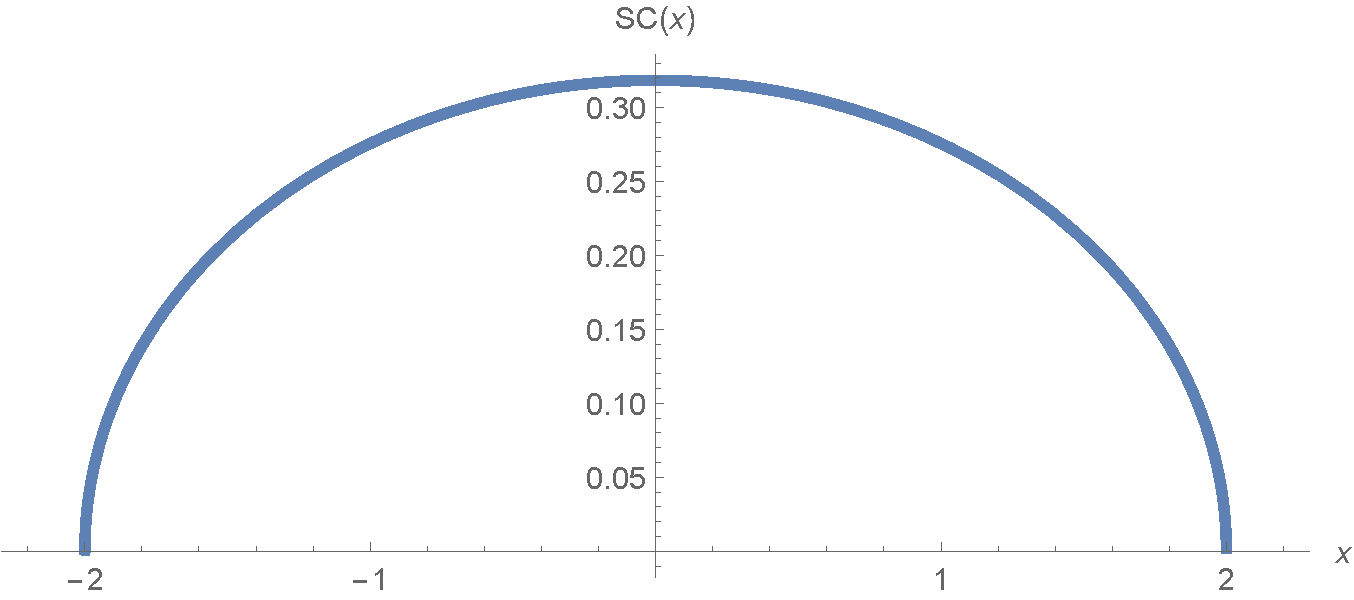
\includegraphics[width=.5\textwidth]{img/SC.pdf}
	\caption{Semicircle density $\SC(x)$.}
	\label{fig:semicircle}
\end{figure}

\begin{theorem}[Wigner's Semicircle Law]\label{thm:SemicircleLaw}
	As $N\to\infty$,
	the empirical distributions 
	$L_N$ converge weakly, in probability to the 
	semicircle distribution $\SC$.
\end{theorem}

\begin{figure}[htbp]
	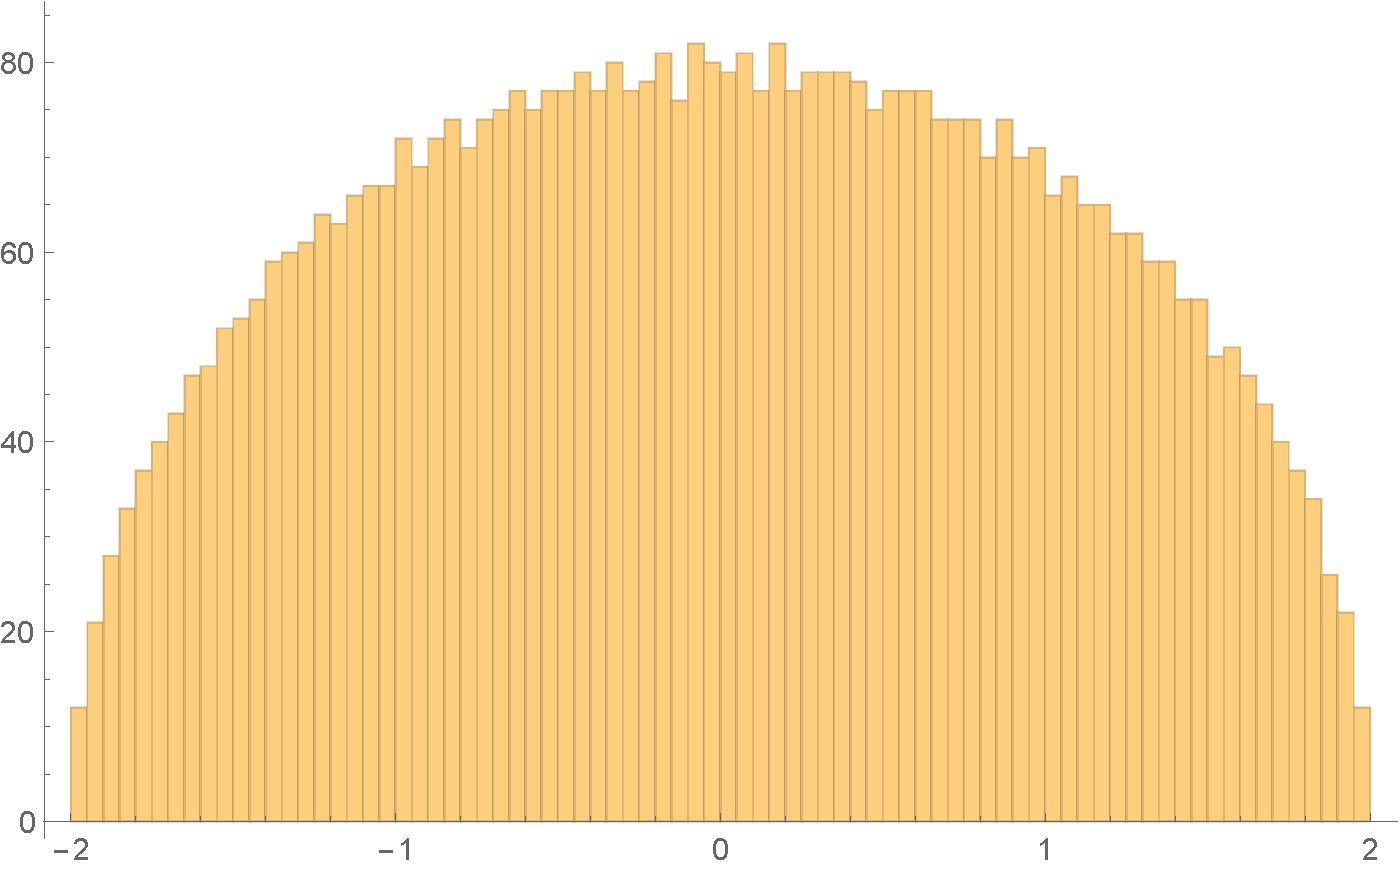
\includegraphics[width=.5\textwidth]{img/Wigner1.pdf}
	\caption{Histogram of the empirical distribution 
	$L_N$ for $N=5000$.}
	\label{fig:Wigner}
\end{figure}

Let us explain what we mean by convergence ``weakly in probability''. Formally this means that
for any bounded continuous function $f$ on $\mathbb R$ ($f\in C_B(\mathbb R)$) and each $\epsilon>0$ we have 
\begin{equation}\label{WignerSemicircleLaw}
\lim_{N\to\infty}\mathbb P\left(\left|\int_{\mathbb R} f\,dL_N-\int_{\mathbb R} f\,d\SC\right|>\epsilon\right)=0.
\end{equation}
That is, ``in probability'' means the usual convergence in probability  of
random elements $L_N$ to a (nonrandom) element $\SC$.  On the other hand,
``weakly'' specifies the metric on the space of probability measures on
$\mathbb{R}$ (to which all $L_N$ and $\SC$ belong). Convergence of probability
measures in this metric simply means weak convergence of probability measures
on $\mathbb{R}$.

In other words,
let us use a convenient notation for the pairing $\langle f,\mu\rangle
=\int_{\mathbb R} f\,d\mu=\int_{\mathbb R}f(x)\,\mu(dx)$ for a given
function $f$ and measure $\mu$.  If $\mu$ is a random measure (such as $L_N$,
since $L_N$ depends on $A_N$ which is random), then $\langle f,\mu\rangle$ is
a random element of $\mathbb R$ (usually we say random variable).  Since $\SC$
is not random, the pairing $\langle f,\SC\rangle$ is a fixed number for a given function $f$.  The
Semicircle Law thus states that for any given $f\in C_B(\mathbb R)$ the random variable
$\langle f,L_N\rangle$ converges in probability to the constant $\langle f,\SC\rangle$ which may be written as
\begin{equation*}
\forall \epsilon>0,\qquad \lim_{N\to\infty}\PP\left(\left|\langle f,L_N\rangle-\langle f,\SC\rangle\right|>\epsilon\right)=0,
\end{equation*}
which is the same as \eqref{WignerSemicircleLaw}.

\begin{remark}
	This type of convergence is reminiscent of the classical weak law of large numbers: for
	$\{X_i\}_{i=1}^\infty$ iid random variables with $\EE|X_1| <\infty$, the random
	variables $\dfrac{1}N\sum_{i=1}^N X_i$ converge to the constant $\EE X_1$ in probability as $N\to\infty$.
\end{remark}

% subsection formulation_of_the_wigner_semicircle_law (end)

\lect{1/25/2016}







% section wigner_s_semicircle_law (end)

\bibliography{bib}
\bibliographystyle{amsalpha}

\end{document}